\section{Signalübertragung}
Um digitale Signale zu übertragen in einem Differenzsignal, sollten sich die Energie von Mark (1) Space (0) maximal unterscheiden.
\[
s_2(t) = -s_1(t)
\]

\subsection{Leitungscodierung}
\subsubsection{Unipolar NRZ, NRZ-L}
\begin{center}
	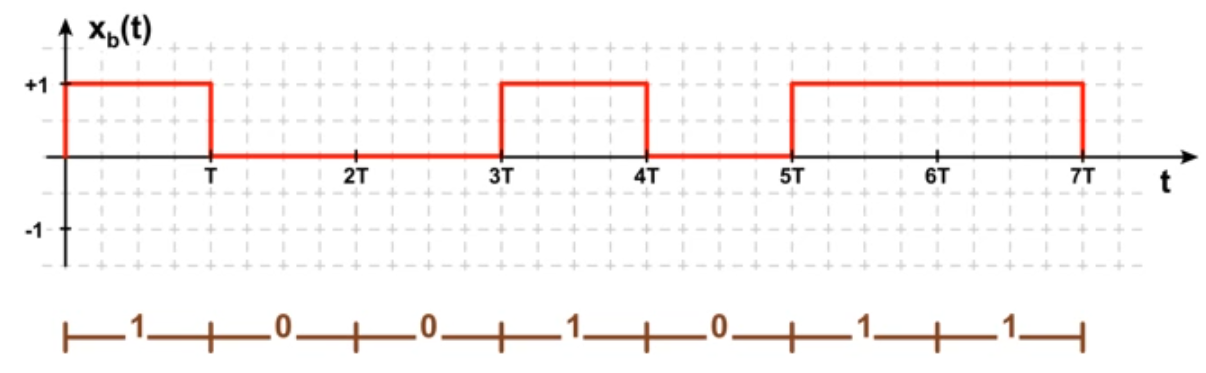
\includegraphics[width=0.6\columnwidth]{Images/nrz}\script{93}
\end{center}
Verbesserung des NRZ können durch \textbf{Scrambling}, \textbf{Bitstopen} oder \textbf{8b/10b-Codierung} erreicht werden.\\

\begin{itemize}[nosep]
	\item \textbf{Mark:} Amplitude A, \textbf{Space:} Amplitude 0
	\item \textbf{Aufwand (De-)Codierung:} sehr klein
	\item \textbf{Taktrückgewinnung:} ohne zusätzliche Codierung unsicher
	\item \textbf{DC-Freiheit:} sehr schlecht, viel DC-Anteil
	\item \textbf{Bandbreitenbedarf:} mittel
\end{itemize}


\subsubsection{Bipolar NRZ}
\begin{center}
	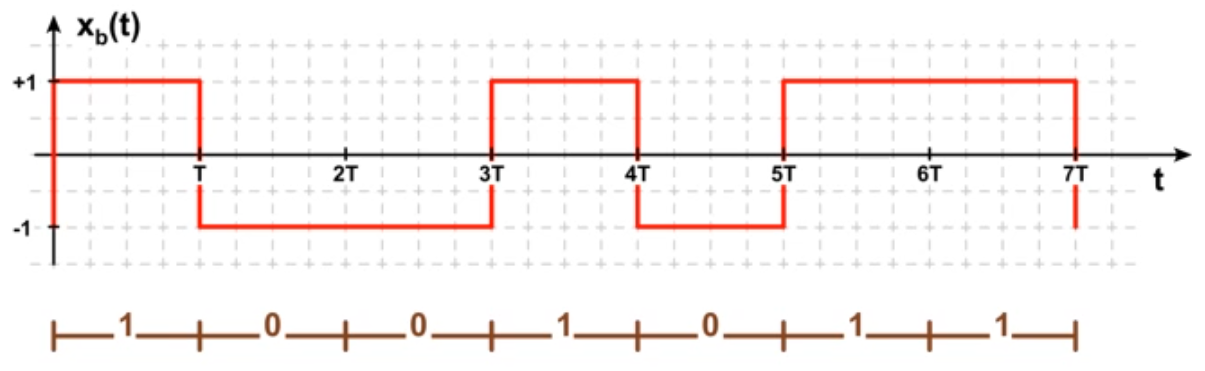
\includegraphics[width=0.6\columnwidth]{Images/nrz1}\script{95}
\end{center}
\begin{itemize}[nosep]
	\item \textbf{Mark:} Amplitude A, \textbf{Space:} Amplitude -A
	\item \textbf{Aufwand (De-)Codierung:} sehr klein
	\item \textbf{Taktrückgewinnung:} ohne zusätzliche Codierung unsicher
	\item \textbf{DC-Freiheit:} Abhängig vom Verhältnis von Mark und Space
	\item \textbf{Bandbreitenbedarf:} mittel (wie unipolares NRZ)
\end{itemize}

\subsubsection{NRZI}
\begin{center}
	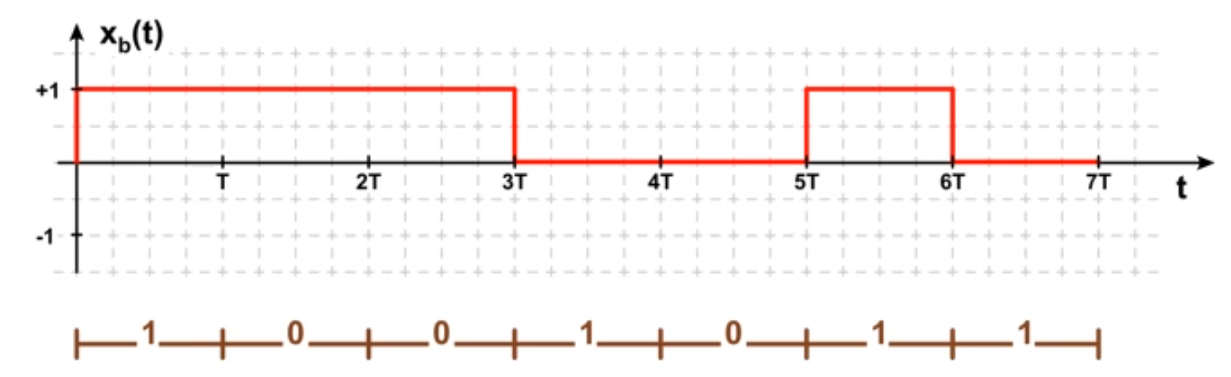
\includegraphics[width=0.6\columnwidth]{Images/nrzi}\script{96}
\end{center}
\begin{itemize}[nosep]
	\item \textbf{Bei NRZI, NRZ-M:} \textbf{Mark:} Amplitudenwechsel, \textbf{Space:} kein Amplitudenwechsel
	\item \textbf{Bei NRZ-S:} \textbf{Mark:} kein Amplitudenwechsel, \textbf{Space:} Amplitudenwechsel
	\item \textbf{Aufwand (De-)Codierung:} gering
	\item \textbf{Taktrückgewinnung:} ohne zusätzliche Codierung unsicher
	\item \textbf{DC-Freiheit:} sehr schlecht, viel DC-Anteil
	\item \textbf{Bandbreitenbedarf:} mittel
\end{itemize}

\subsubsection{Unipolar RZ}
\begin{center}
	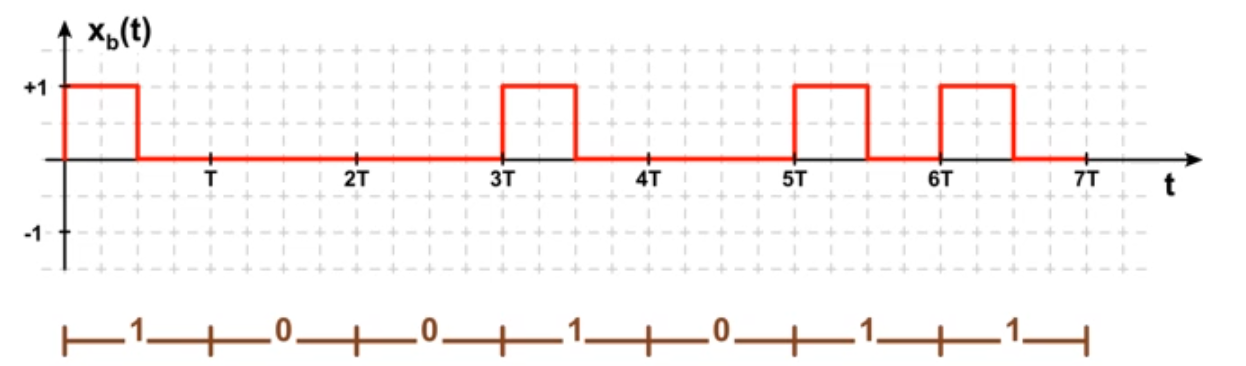
\includegraphics[width=0.6\columnwidth]{Images/urz}\script{97}
\end{center}
\begin{itemize}[nosep]
	\item \textbf{Mark:} Amplitude A (nach halber Bitzeit 0), \textbf{Space:} Amplitude 0
	\item \textbf{Aufwand (De-)Codierung:} gering
	\item \textbf{Taktrückgewinnung:} besser als NRZ, Space-Folgen immer noch heikel
	\item \textbf{DC-Freiheit:} sehr schlecht, viel DC-Anteil
	\item \textbf{Bandbreitenbedarf:} grösser als NRZ
\end{itemize}

\subsubsection{Bipolar RZ}
\begin{center}
	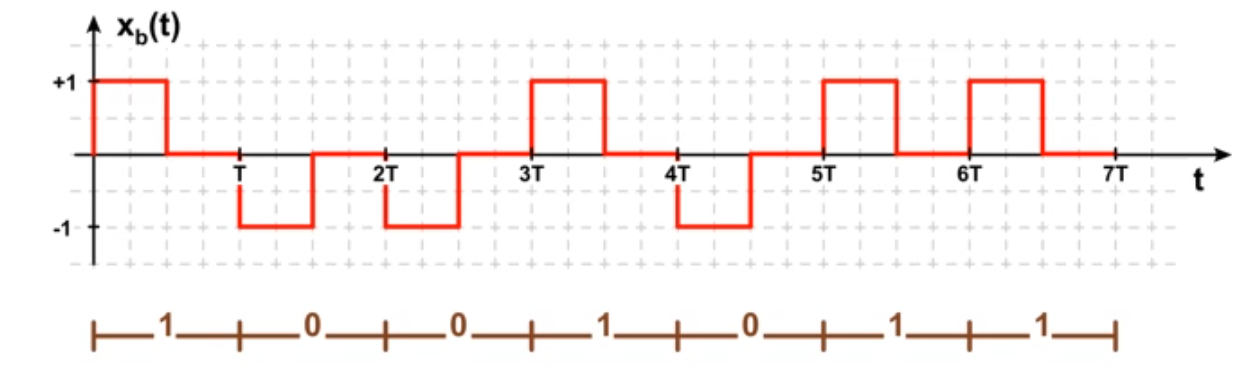
\includegraphics[width=0.6\columnwidth]{Images/brz}\script{97}
\end{center}
	\begin{itemize}[nosep]
	\item \textbf{Mark:} Amplitude A (nach halber Bitzeit 0), \textbf{Space:} Amplitude -A (nach halber Bitzeit 0)
	\item \textbf{Aufwand (De-)Codierung:} mittel
	\item \textbf{Taktrückgewinnung:} sehr gut
	\item \textbf{DC-Freiheit:} Abhängig vom Verhältnis von Mark und Space
	\item \textbf{Bandbreitenbedarf:} grösser als NRZ
	\item pseudoternäres Signal
\end{itemize}

\subsubsection{AMI}
\begin{center}
	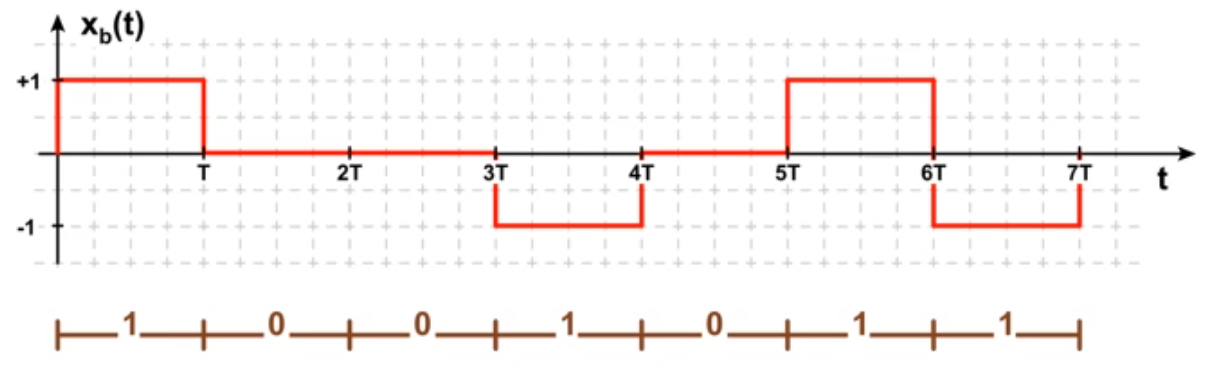
\includegraphics[width=0.6\columnwidth]{Images/ami}\script{98}
\end{center}
\begin{itemize}[nosep]
	\item \textbf{Mark, Space:} Wie unipolares NRZ, doch mit alternierenden Amplituden $\pm$A für Mark
	\item \textbf{Aufwand (De-)Codierung:} mittel
	\item \textbf{Taktrückgewinnung:} besser als NRZ, Space-Folgen immer noch heikel
	\item \textbf{DC-Freiheit:} sehr gut
	\item \textbf{Bandbreitenbedarf:} sehr schlecht, viel DC-Anteil
	\item pseudoternäres Signal
\end{itemize}

\subsubsection{Manchester Code}
\begin{center}
	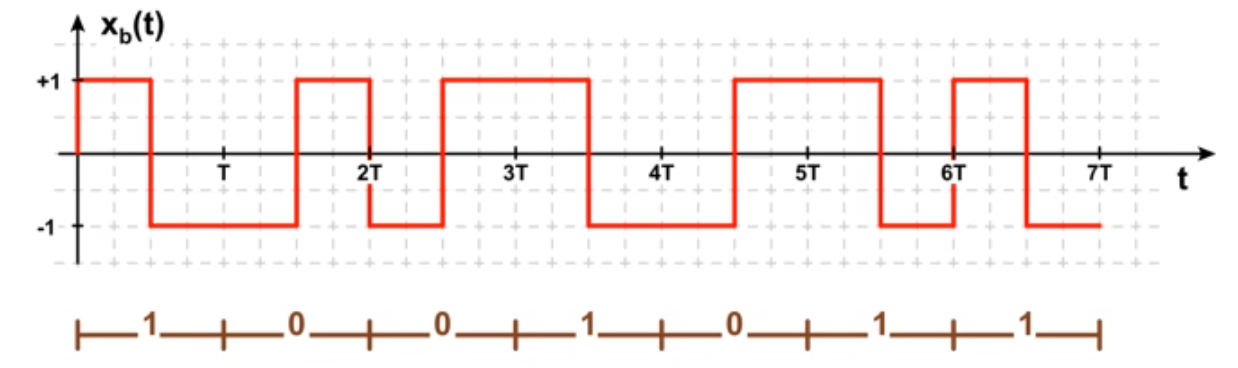
\includegraphics[width=0.6\columnwidth]{Images/manchester}\script{99}
\end{center}
\begin{itemize}[nosep]
	\item \textbf{Mark:} Übergang in Symbolmitte von +A nach -A, \textbf{Space:} Übergang in Symbolmitte von -A nach +A
	\item \textbf{Aufwand (De-)Codierung:} mittel
	\item \textbf{Taktrückgewinnung:} sehr gut
	\item \textbf{DC-Freiheit:} sehr gut
	\item \textbf{Bandbreitenbedarf:} grösser als NRZ
	\item pseudoternäres Signal
\end{itemize}

\subsubsection{MLT3}
\begin{center}
	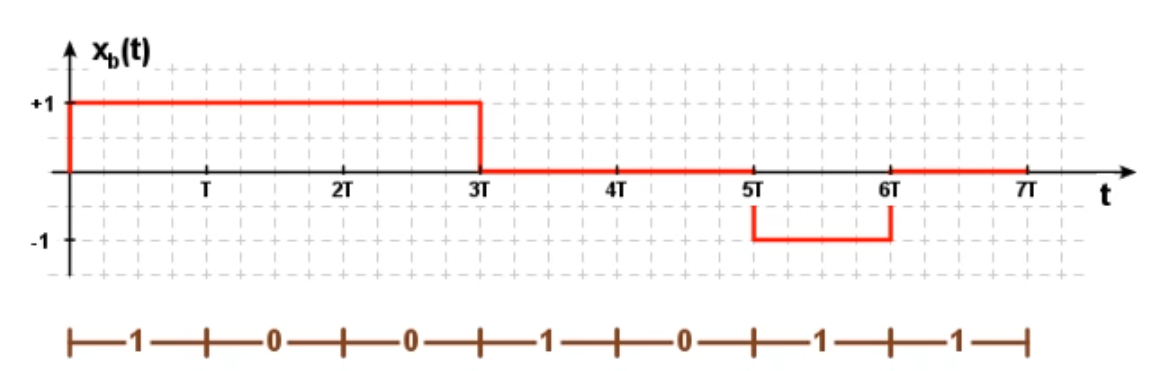
\includegraphics[width=0.6\columnwidth]{Images/mlt3}\script{99}
\end{center}
\begin{itemize}[nosep]
	\item Pseudoternäres Signal mit 3 Amplitudenwerten +A, 0, -A (\textbf{Mark:} Amplitudenübergang, \textbf{Space:} konstante Amplitude)
	\item \textbf{Ablauf der Übergänge:} 0, +A, 0, -A, 0, +A, 0 etc.
	\item \textbf{Taktrückgewinnung:} heikel bei langen Space-Folgen
	\item \textbf{DC-Freiheit:} heikel bei langen Space-Folgen
	\item \textbf{Bandbreitenbedarf:} ca. halb so gross wie NRZ
\end{itemize}

\subsubsection{PAM5}
\begin{center}
	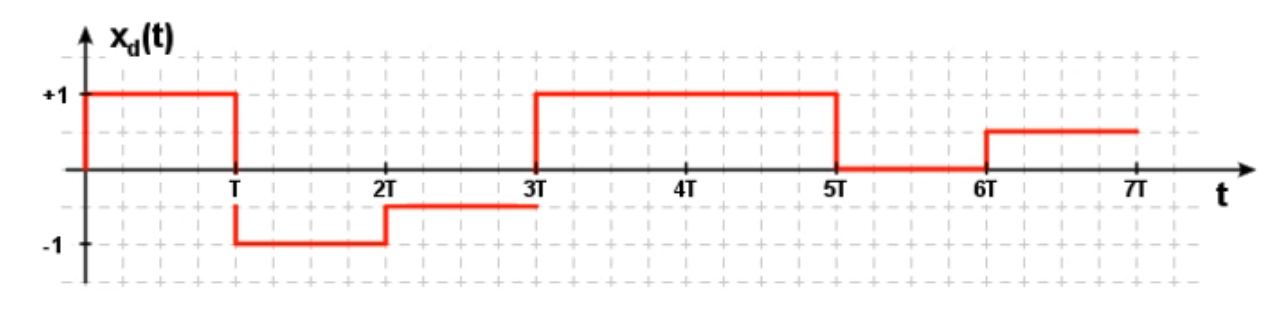
\includegraphics[width=0.6\columnwidth]{Images/pam5}\script{101}
\end{center}
\begin{itemize}[nosep]
	\item Mehrwertiges Signal mit fünf Amplitudenwerten: +A, +A/2, 0, -A/2, -A
	\item \textbf{Ablauf der Übergänge:} 0, +A, 0, -A, 0, +A, 0 etc.
	\item \textbf{Taktrückgewinnung:} heikel bei langen Space-Folgen
	\item \textbf{DC-Freiheit:} heikel bei langen Space-Folgen
	\item \textbf{Bandbreitenbedarf:} ca. halb so gross wie NRZ
\end{itemize}

\subsection{Bandbreitenbedarf}\script{102}
Der minimale Bandbreite $B_d$ [Hz] kann abgeschätzt werden mit $B_d = \frac{f_s}{2}; f_s = \frac{1}{T_s}$

\subsection{Äquivalente Basisbanddarstellung von Bandpasssignalen} 
Bei QAM werden zB für QAM-16 $2^n \rightarrow n = 4Bit/Symbol$ übertragen. Somit werden für Datenrate $d =10kBit/s$ $\frac{d}{n} = 2500Symbole/s$ übertragen \script{114}\\
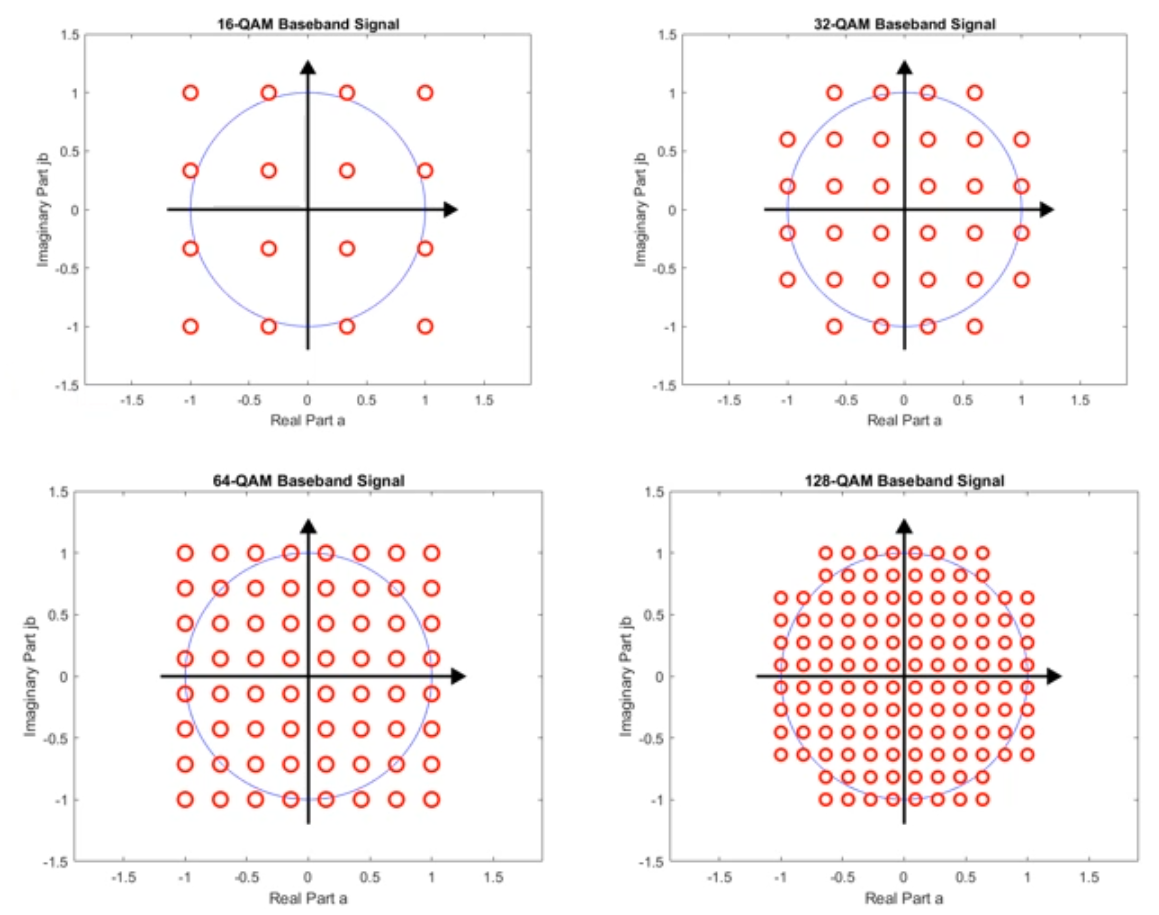
\includegraphics[width=\columnwidth]{Images/qam_basisdarstellung}

\subsection{Pulsformfilter}\script{104}
Um Bandbreite bei der Übertragung einzusparen, werden Rechtecks Signale, wie sie bei der PCM (Pulse-Code-Modulation) vorkommen, schon beim Sender mit einem Filter Abgeflacht, dadurch hat man die physikalische Bandbreite des Kanals unter eigener Kontrolle.

\subsubsection{Raised-Cosine Puls}
Ein beliebter Pulseformfilter ist Raised-Cosine Pulse \script{105} welcher definiert ist durch 
\[
h(t) = \sinc\left(\frac{\pi}{T}t\right)\cdot\frac{\cos(\alpha\frac{\pi}{T}t)}{1- (\frac{2\alpha\pi}{T}t)^2}
\]
Dadurch lassen sich die spektral Bandbreite beschränken und trotzdem beleibt die übertragenen Pulse zum optimalen Zeitpunkt der Auswertung frei von Intersymbol-Interferenz.
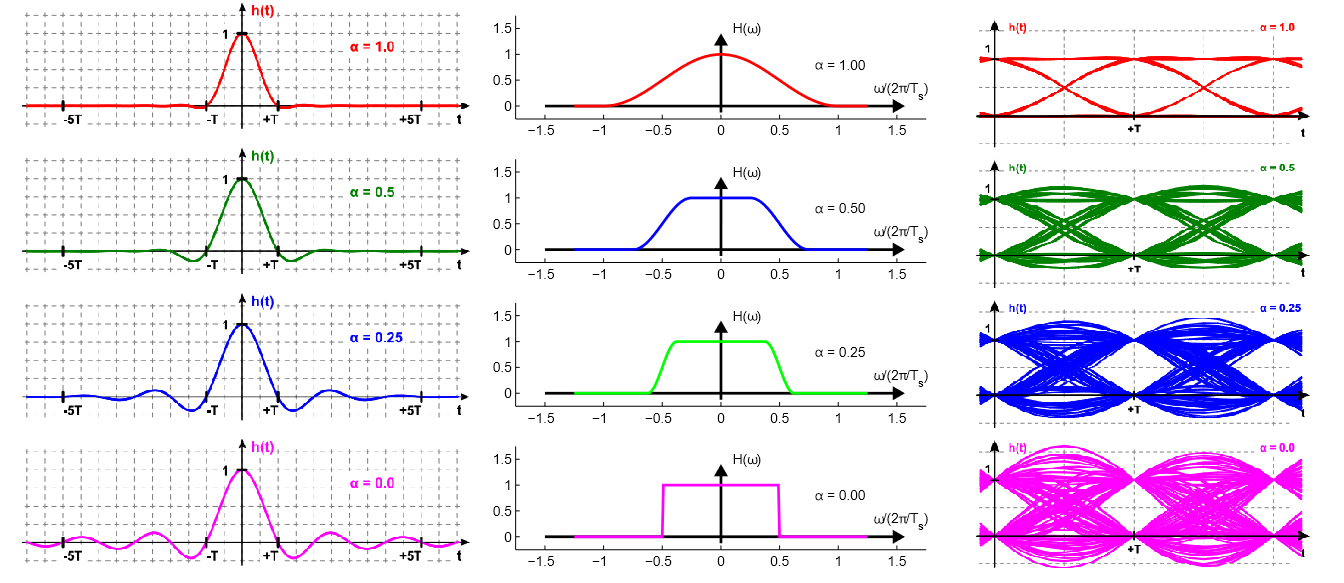
\includegraphics[width=\columnwidth]{Images/raised-cosine_pulse}
Die \textbf{Symbolrate} mit gegebenen Roll-off-Faktors $\alpha$ und einer Bandbreite $B$, dabei ist die Übertragungsrate maximal bei $\alpha=0$ und minimal bei $\alpha=1$ 
\[
d = \frac{2B}{1 + \alpha}
\]
\textbf{Beispiel}
Die Nutzdaten mit $10MHz$ bei 8b/10b-codierten NRZ-Signal sind $d_d = d \cdot \frac{8}{10} = 16MBit/s$, bei Manchester-Code $d_d = d \cdot \frac{1}{2} = 10MBit/s$

\subsection{Digitale Trägermodulation}
Weil Binäre Nachrichtensignale selbst zu kleine Frequenzen aufweisen, sind sie nicht geeignet um über den Äther zu schicken. Die binäre Trägermodulation kann dabei Helfen um physikalische Anpassungen an Kanal vorzunehmen, die 
Mehrfachnutzung des Kanals und erhöht die Störfestigkeit.\script{109}

Dabei gibt es folgende Möglichkeiten
\begin{itemize}[nosep]
	\item Amplituden Shift Keying (ASK)
	\item Phase Shit Keying (PSK)
	\item Frequency Shit Keying (FSK)
\end{itemize}